Cette fonction, accessible via le menu Algorithms, permet d'afficher les segments ressemblants entre deux dump sous forme de graphe. Il faut en premier lieu cliquer sur Dot Plot Pattern dans le menu Algorithms. Une fenètre s'affiche alors :

\begin{figure}[!h]
  \begin{center}
  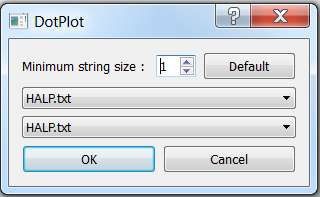
\includegraphics[scale=1]{dotplotdialog.png}
  \caption{Fenetre de lancement du Dot Plot Pattern}
  \label{dotplotdialog}
  \end{center}
\end{figure}

Il faut alors sélectionner une \emph{Minimum String Size}; il s'agit de la taille minimale que les blocs de données identiques doivent avoir pour apparaitre. Si vous avez peu de diagonales sur votre Dot Plot Pattern, c'est peut-être que vous avez sélectionné une taille de diagonale trop grande. Le bouton \emph{Default} permet d'entrer une taille qui promet statistiquement de bons résultats.
Les deux champs suivant permettent de sélctionner les deux dumps qui seront utilisés lors du Dot Plot Pattern. Le premier dump se retrouvera en abscisse, et le second en ordonnée. Il est possible d'utiliser deux fois le même dump, pour voir les motifs se répétant au sein d'un même dump.

Après appui sur le bouton \emph{OK}, on obtient la fenètre suivante :
\begin{figure}[!h]
  \begin{center}
  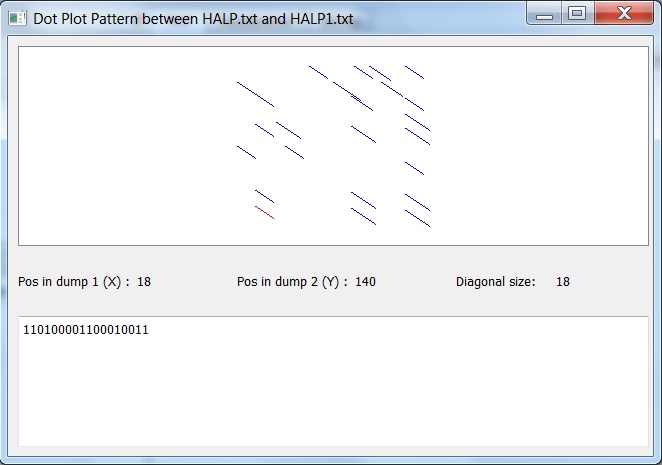
\includegraphics[scale=1]{dotplotpatternview.png}
  \caption{Fenetre du Dot Plot Pattern}
  \label{dotplotpattern}
  \end{center}
\end{figure}

Un click sur une diagonale la sélectionne; elle devient rouge et le bas de l'interface est actualisée avec les informations relative à celle-ci :
\begin{description}
\item[Pos in dump 1 (X)] \hfill \\
	Indique le numéro du bit où commence la ressemblance dans le premier dump, 0 correspondant au début de fichier.
	
\item[Pos in dump 2 (Y)] \hfill \\
	Indique le numéro du bit où commence la ressemblance dans le deuxième dump, 0correspondant au début de fichier.

\item[Diagonal Size] \hfill \\
	Indique la longueur de la diagonale, ce qui correspond au nombre de bits en commun de suite entre les deux dumps.
	
\item[La zone de texte en bas] \hfill \\
	Elle contient la chaine de bits commune aux deux dumps.

\end{description}

Si les deux dumps disposent de champs identiques aux mêmes endroits, il y a alors des diagonales au centre du graphe. Si les deux dumps sont identiques, alors une diagonale centrale faisant la longueur du dump est visible.